\subsection{Part 3 forecast audit and scientific gate}
The eight common recordings and all model workers complete normally. The forecast
audit fails accuracy, with every support requirement satisfied; the physical
64-episode optimizer comparison is therefore unstarted by protocol. No Part 3
finalist, lineage, optimizer outcome or superiority result is asserted. This is a
measured negative feasibility result, not a time-limited incomplete stage.

The corpus has sixteen fitting, four calibration and four audit episodes. Audit
contains 552 four-action query-start windows, of which 263 exceed the fitting
median displacement, 101 are near the upright boundary and 99 end with negative
margin. Near-boundary events occur in four calibration and two audit episodes,
with one audit episode crossing the boundary. There are 152 varying-progress
windows. Windows are correlated within four episodes on one held-out task; they
are not 552 independent safety trials.

On changing windows, one-action error is .2962 for the ensemble versus .2318 for
persistence. Four-action errors are .4120 for persistence, .5179 for ridge, .5214
for action-shuffled fitted ridge, .6145 for the same ensemble with shuffled action
prefixes and .5979 for correctly paired actions (Figure~\ref{fig:part3-forecast}).
The ensemble is 27.8\% and 45.1\% worse than persistence at one and four actions.
Its 2.69\% improvement over mispaired actions passes the action-dependence check,
but does not compensate for absolute/reference failures (Table~\ref{tab:forecast}).
The actual-state head also fails before dynamics prediction is introduced.

\begin{figure*}[t]
\centering
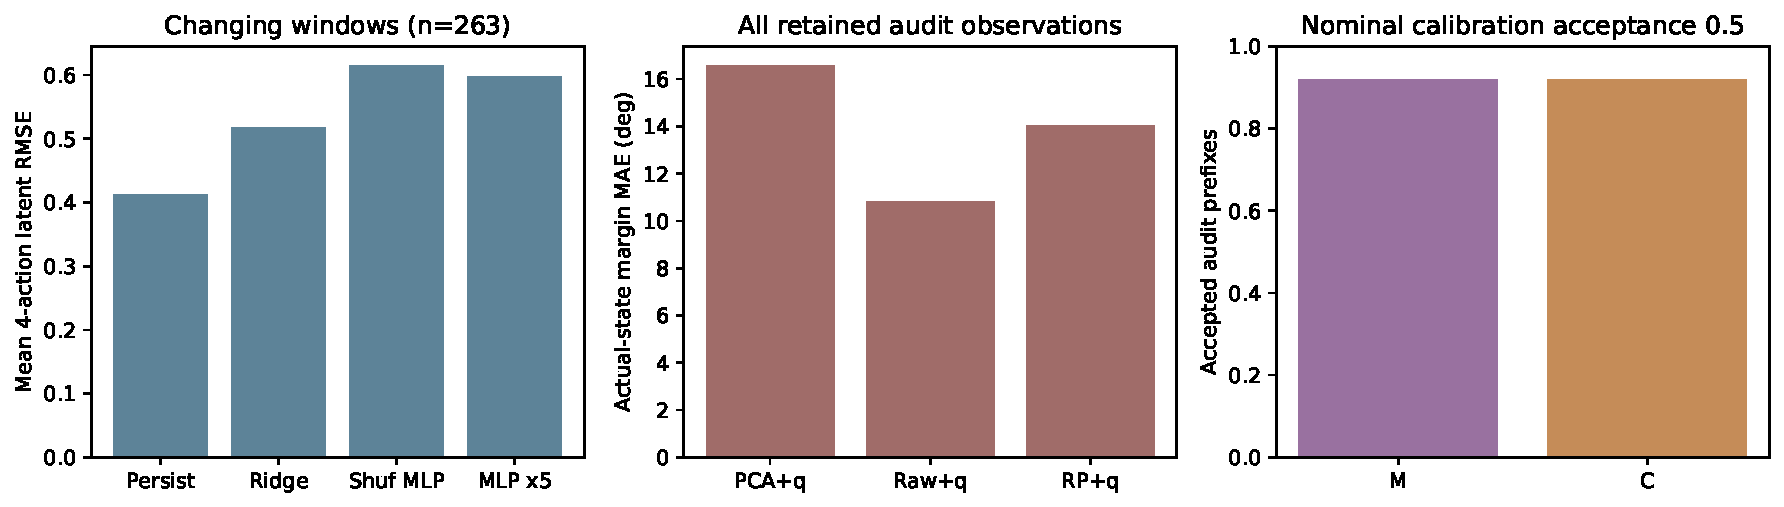
\includegraphics[width=\textwidth]{part3-forecast.pdf}
\caption{Part 3 forecast audit. Left: mean per-window standardized visual-latent RMSE
on 263 changing windows. The shuffled-prefix control uses the same ensemble.
Middle: actual-state readouts on every retained audit observation, with robot state
included. Right: actual acceptance over all 552 audit prefixes. These quantities
are not safety probabilities.}
\Description{The ensemble is worse than persistence and ridge. Raw features improve
the combined readout relative to PCA, while both trust methods accept about 92 percent.}
\label{fig:part3-forecast}
\end{figure*}

\begin{table}[t]
\caption{Frozen forecast criteria and observed values. All event-support criteria
pass; seven accuracy/usefulness criteria fail. Degrees and millimetres are physical
readout errors; latent errors use standardized coordinates.}
\label{tab:forecast}
\begin{tabular}{lrr}
\toprule
Criterion & Measured & Required \\
\midrule
One-step improvement & $-27.8\%$ & $\ge5\%$ \\
Four-step improvement & $-45.1\%$ & $\ge5\%$ \\
Shuffled-prefix improvement & $2.69\%$ & $\ge2\%$ \\
Ensemble/ridge error & 1.155 & $\le1.05$ \\
Actual-state margin MAE & $16.17^\circ$ & $\le10^\circ$ \\
Near-boundary forecast MAE & $18.56^\circ$ & $\le10^\circ$ \\
Progress MAE & 79.01 mm & $\le30$ mm \\
Progress ranking, Spearman & .126 & $\ge.25$ \\
False reassurance & 0/99 & $\le.10$ \\
M/C actual acceptance & 507/552 & $\ge.10$ \\
Sixteen-candidate screening & .810 s & $\le30$ s \\
\bottomrule
\end{tabular}
\end{table}

All 818 calibration prefixes fall below the first .5 correction boundary, with
maximum .17839. Sparse-bin fallback makes every conditional error quantile equal
to .80913. C is then a positive affine transform of M; the same support conditions
and transformed median thresholds produce exactly equal audit acceptance masks:
507/552 each, or 91.85\%, versus 50\% on calibration (Figure~\ref{fig:calibration}).
Audit bins contain 551/1/0/0/0/0 prefixes. This calibration supplies no distinct
correction-dependent allocation rule. It is retained rather than repaired using
held-out outcomes. Zero false reassurance among 99 correlated negative-margin
windows from one episode does not validate a safety guarantee.

\begin{figure*}[t]
\centering
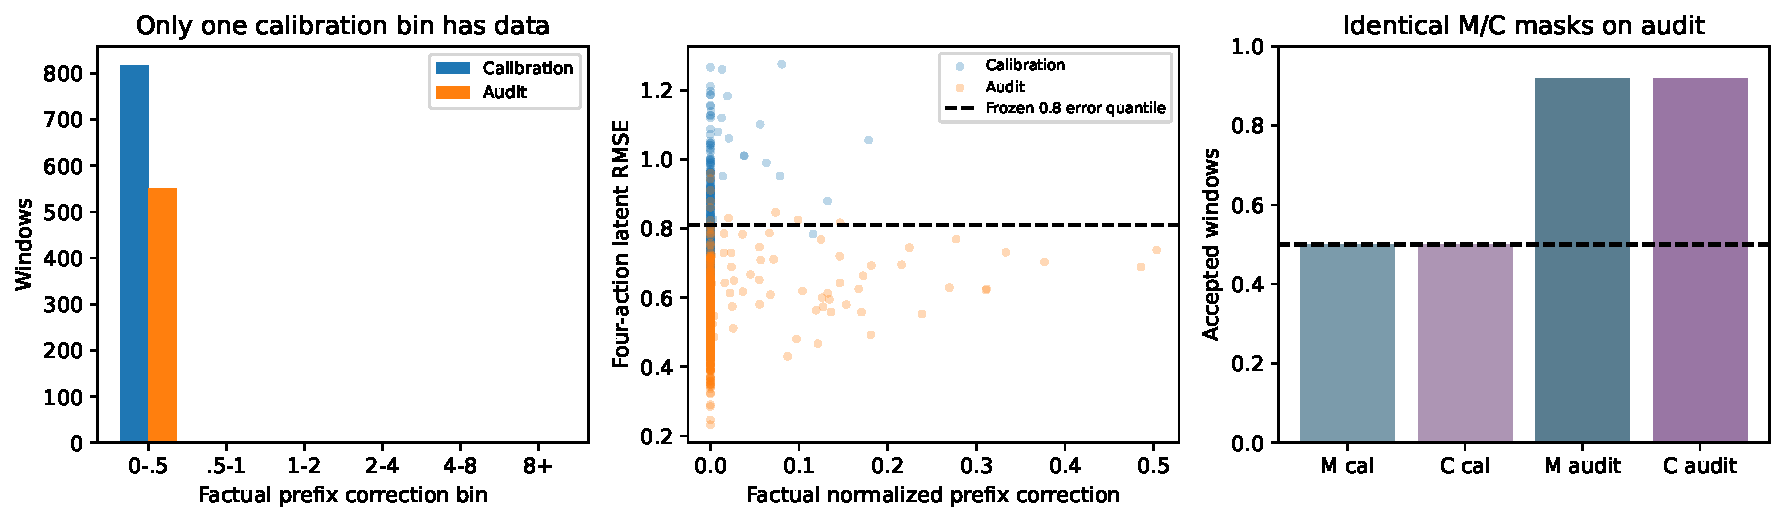
\includegraphics[width=\textwidth]{part3-calibration.pdf}
\caption{The frozen correction calibration collapses to one populated bin. Empty
bins use the unconditional .8-error quantile. M and C have equal acceptance masks,
and their nominal calibration acceptance does not persist on the audit task. No
additional episode or changed threshold follows this result.}
\Description{All calibration data occupy the first correction bin. The constant
error lookup makes correction-dependent trust equivalent to disagreement trust.}
\label{fig:calibration}
\end{figure*}

A post hoc, frozen-weight diagnostic matches every head on the same 552 actual
future observations. Margin MAE is $16.17^\circ$ for PCA plus robot state,
$11.03^\circ$ for raw pooled features plus robot state, $12.82^\circ$ for a random
projection plus robot state, and $8.54^\circ$ for visual-only PCA. Their progress
errors are 80.57/52.94/104.53/41.13 mm. The visual-only contrast motivates testing
cross-task covariate conditioning; it prevents diagnosing PCA information loss
alone as the established cause. No head is replaced after audit. Fitting PCA
retains 82.05\% of visual variance, without certifying task/safety information.

The common recordings yield 3/8 safe completions, 4/8 violations and 5/8 unfinished
episodes, with no unsafe completion. Calibration has 0/4 completions and three
violations; audit has three safe completions and one violation. These data-acquisition
outcomes are not an evolutionary comparison. Both native cameras, eight matched
recording videos and complete event/episode picture strips are preserved.
